\videotitle{Meta-Learning}
%----------------------------------------------------------------------

\begin{frame}[c]{Introduction}

	\begin{center}
		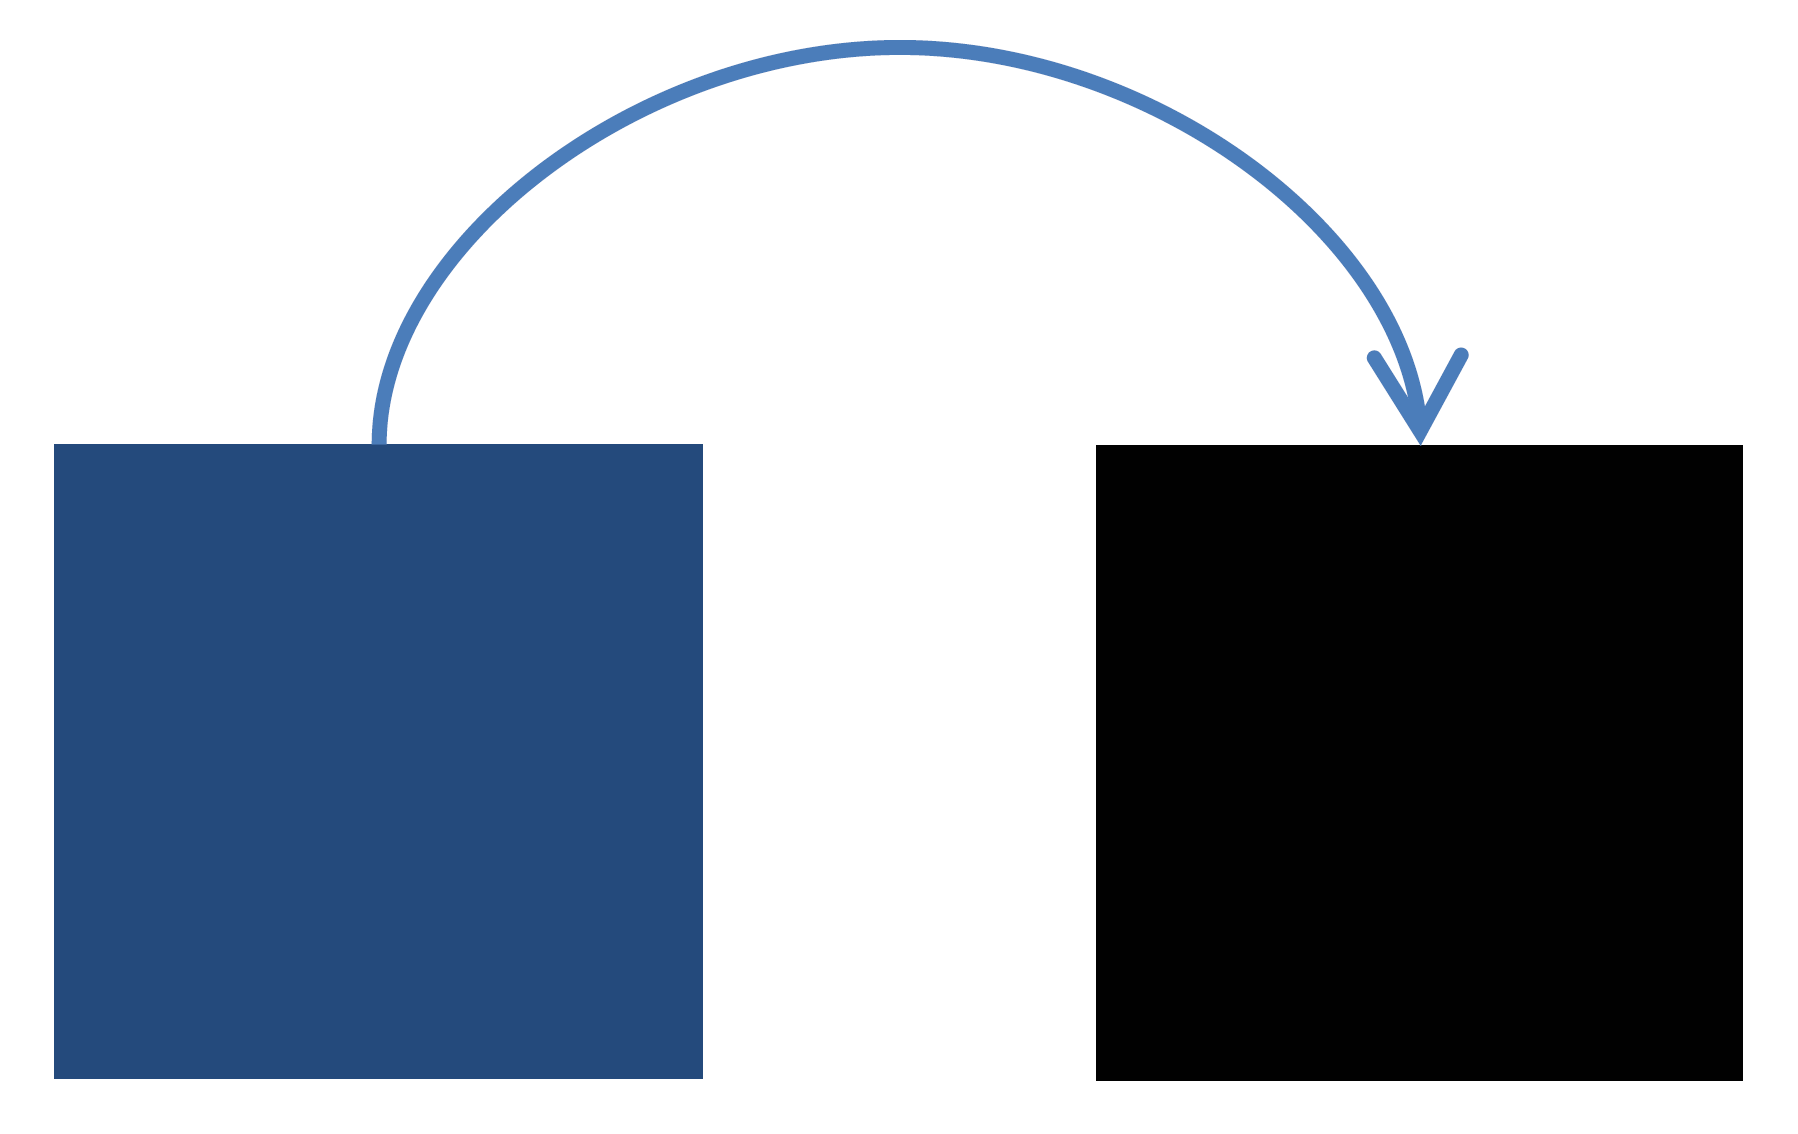
\includegraphics[width=0.2\linewidth, keepaspectratio=true]{images/intro/meta-learning.png}
	\end{center}
				
	\begin{itemize}
		\item Learning essentially never stops:
		\begin{itemize}
			\item Many models are periodically re-fit to track changes in the data
			\item Many models are re-fit to perform well on new tasks
		\end{itemize}
		\item The best hyperparameter configuration tends to remain quite stable across tasks
	\end{itemize}
	\bigskip
	\bigskip
	\bigskip
\pause
	\begin{center}
	For a good introduction to meta-learning in general, see \lit{\href{https://www.springer.com/gp/book/9783030053178}{AutoML Book: Chapter 2}}
	\end{center}			
\end{frame}

\begin{frame}[c]{Problem Statement}
%	\myblock{Definition: meta-learning for HPO}{
		Given:
	    \myit{
	        \item a set of prior tasks: 
	        %(e.g., datasets): 
	        $t_{j} \in \mathcal{T}_{\text{meta}} \subset \mathcal{T}$,
	        \item a set of new tasks: 
	        %(e.g., datasets): 
	        $t_{\text{new}} \in \mathcal{T}$,
\pause
	        \item a set of learning algorithms, fully defined by $\theta_{i} \in \Theta$
\pause
	        \item a set of prior evaluations $\dataset_{\text{meta}}$ on $t_j \in \mathcal{T}_{\text{meta}}$%, where $\dataset_{i, j} = \cost(\theta_{i}, t_{j})$
	        \item a set of evaluations $\dataset_{\text{new}}$ on new task $t_{\text{new}}$
		}
		\bigskip
\pause
		\alert{Goal of meta-learning:}
		\myit{
			\item use meta-data $\mathcal{D}_{\text{meta}}$ to choose $\theta_{i} \in \Theta$ for $t_{\text{new}}$ better than only based on $\dataset_{\text{new}}$. 
		}
%	}	
\bigskip
\hspace{9cm}\lit{adapted from \href{https://www.springer.com/gp/book/9783030053178}{AutoML Book: Chapter 2}}
\end{frame}


% %----------------------------------------------------------------------
% %----------------------------------------------------------------------
% \begin{frame}[c]{Meta-Learning}
% \framesubtitle{Introduction}

% \begin{columns}
% 	\column{0.18\textwidth}
% 	Ren\'e Magritte
% 	\centering
% 	
\includegraphics[width=.9\textwidth]{../w07_hpo_speedup/images/meta_learning/magritte_1.jpg}
% 	
\includegraphics[width=.9\textwidth]{../w07_hpo_speedup/images/meta_learning/magritte_2.jpg}
% 	\column{0.258\textwidth}
% 	Francis Picabia
% 	\centering
% 	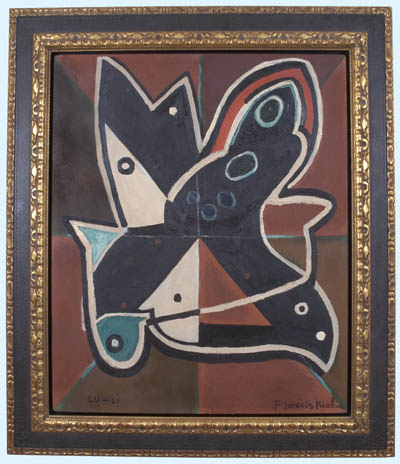
\includegraphics[width=.7\textwidth]{../w07_hpo_speedup/images/meta_learning/picabia_3.jpg}
% 	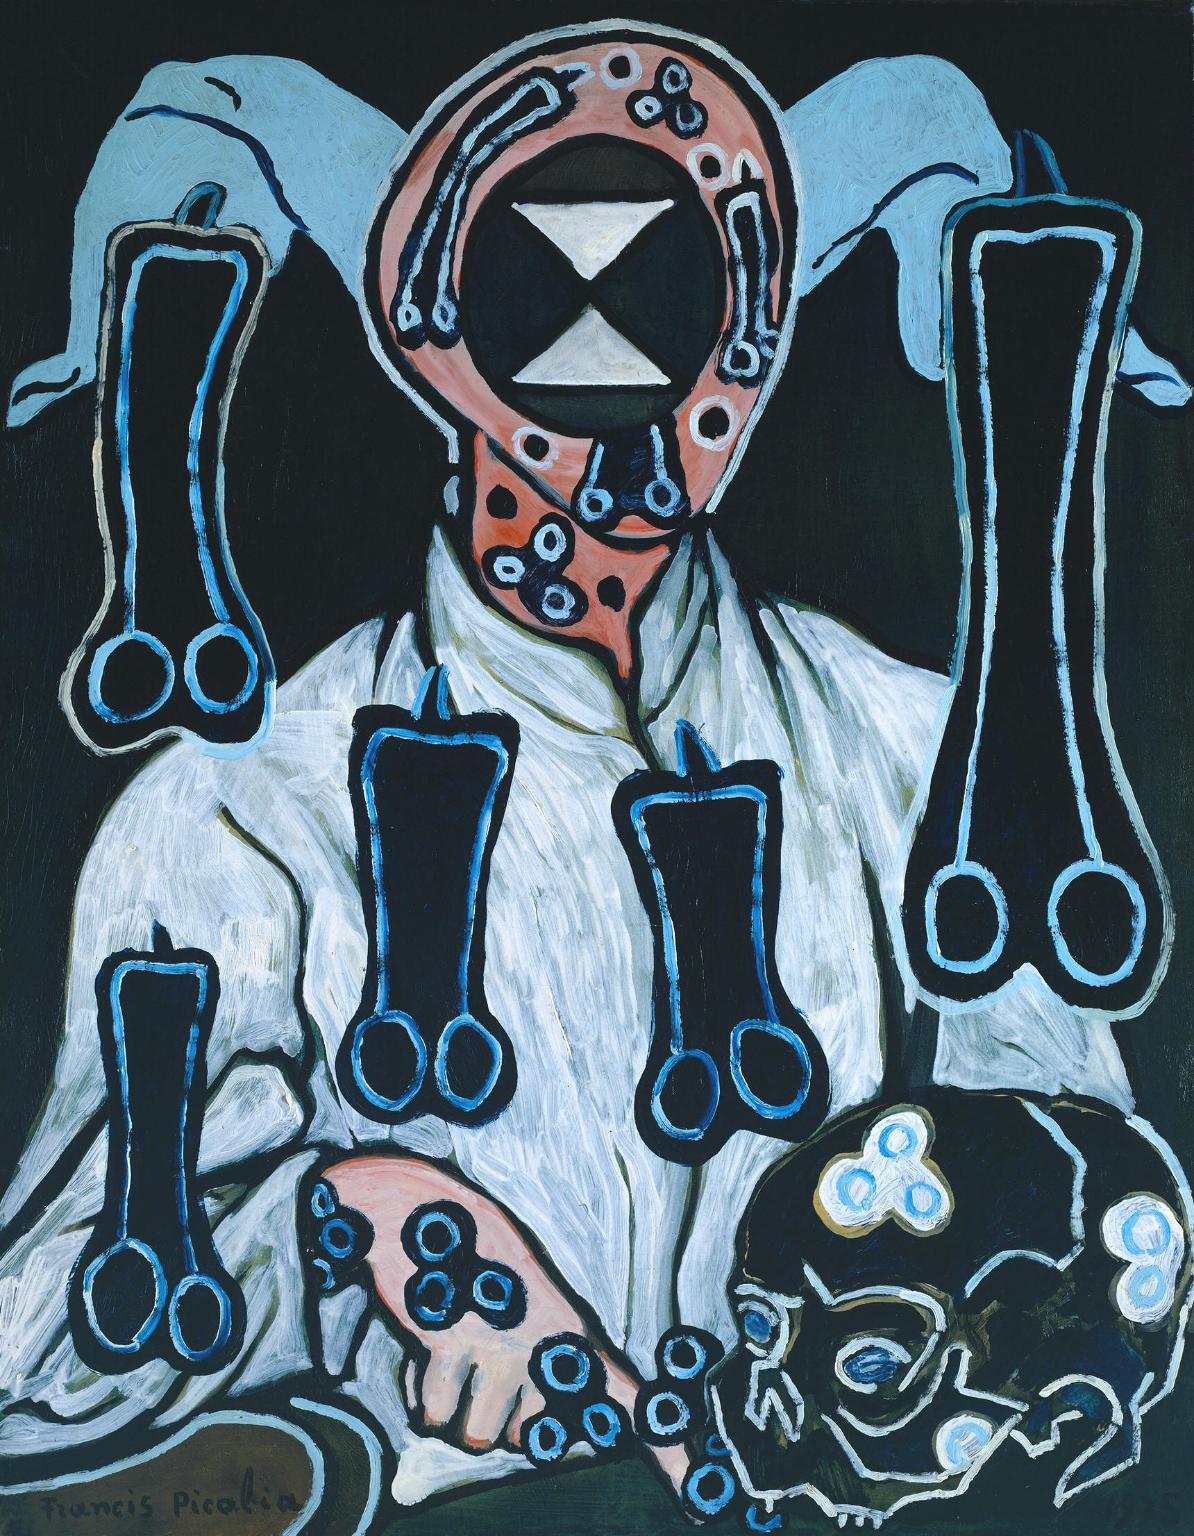
\includegraphics[width=.6\textwidth]{../w07_hpo_speedup/images/meta_learning/picabia_1.jpg}
% 	\column{0.3\textwidth}
% 	\centering
% 	Who painted that?
% 	
\includegraphics[width=.7\textwidth]{../w07_hpo_speedup/images/meta_learning/magritte_3.jpg}
	
% 	\pause
% 	Most likely most of you can identify the painter correctly, 
% 	although I presented only two pictures of each.
% \end{columns}

% \end{frame}
% % %----------------------------------------------------------------------
% % %----------------------------------------------------------------------

%----------------------------------------------------------------------
%----------------------------------------------------------------------
%\begin{frame}[c]{Learning from model evaluations}
%
%\begin{itemize}
%    \item Similarly, while building ML models for a specific task, we exploit our experience with related tasks
%    \item The challenge of meta-learning is to provide a systematic and data-driven approach to learn from experience 
%\end{itemize}
%
%\hspace{11cm}\lit{\href{https://www.springer.com/gp/book/9783030053178}{AutoML Book: Chapter 2}}
%
%\end{frame}
% %----------------------------------------------------------------------
% %----------------------------------------------------------------------

%----------------------------------------------------------------------
%----------------------------------------------------------------------
\begin{frame}[c]{The Role of Meta-Features}

\begin{itemize}
    \item We can often extract additional characteristics for each task, called \alert{meta-features}
    \item Each task $t_j$ can be described by a vector of $K$ meta-features:
        \begin{equation*}
            m(t_j) = (m_{j, 1}, \dots, m_{j, K})
        \end{equation*}
\medskip
\pause
    \item This vector can be used to define a \alert{similarity measure} between two tasks
    \myit{
    	\item e.g., calculating the Euclidean distance between $m(t_i)$ and $m(t_j)$
    }
\smallskip
    \item Based on similarity, we can transfer information from the most similar tasks to the new task $t_{\text{new}}$
    \end{itemize}

\end{frame}
% %----------------------------------------------------------------------
% %----------------------------------------------------------------------

% \begin{frame}[c]{Meta-Learning}
% \framesubtitle{Supervised Learning revisited}

% Dataset:
% \begin{equation*}
% \dataset = \{(x_1, y_1), \ldots, (x_k, y_k) \}
% \end{equation*}

% \bigskip
% \pause

% Learning a model $\phi$ (e.g., weights of a neural network):
% \begin{eqnarray*}
% \argmax_{\phi} \log p(\phi|\dataset)\\
% \pause
% = \argmax_{\phi} \log p(\dataset | \phi) + \log p(\phi) \\
% \pause
% = \argmax_{\phi} \sum_i \log p(y_i | x_i, \phi) + \log p(\phi)
% \end{eqnarray*}

% \pause

% Challenge:
% \begin{itemize}
% 	\item Learning starts from scratch
% 	\item We might only have very few examples in $\dataset$ 
% \end{itemize}

% \end{frame}
% %----------------------------------------------------------------------
% %----------------------------------------------------------------------
% \begin{frame}[c]{Meta-Learning}
% \framesubtitle{Problem formulation}

% Dataset:
% \begin{equation*}
% \dataset = \{(x_1, y_1), \ldots, (x_k, y_k) \}
% \end{equation*}
% Set of datasets (meta-datasets):
% \begin{equation*}
% \mdata = \{\mathcal{D}_1, \ldots, \mathcal{D}_n, \}
% \end{equation*}

% \pause
% Can we include these meta-datasets to improve learning on $\dataset$?
% \begin{equation*}
% \argmax_{\phi} \log p(\phi|\dataset, \mdata)
% \end{equation*}

% \pause
% \medskip

% \alert{Idea:} Instead of keeping $\mdata$ forever, we want to distill the knowledge into \alert{meta-parameters $\theta$}: $p(\theta|\mdata)$
 
% \end{frame}
% %----------------------------------------------------------------------
% %----------------------------------------------------------------------
% \begin{frame}[c]{Meta-Learning}
% \framesubtitle{Problem formulation}

% In meta-learning, we want to learn:
% \begin{eqnarray*}
% \argmax_{\phi} \log p(\phi|\dataset, \mdata) \\
% \pause
% = \argmax_{\phi} \log \int_{\Theta} p(\phi \mid \dataset, \theta) p(\theta \mid \mdata) d\theta\\
% \pause
% \approx \argmax_{\phi} \log p(\phi | \dataset, \theta^*) + \log p(\theta^* | \mdata)\\
% \pause
% = \argmax_{\phi} \log p(\phi | \dataset, \theta^*)
% \end{eqnarray*}

% \pause

% \begin{center}
% \begin{minipage}{0.5\textwidth}
% \begin{block}{Meta-learning problem}
% \begin{equation*}
% \theta^* \in \argmax_{\theta} \log p(\theta | \mdata)
% \end{equation*}
% \end{block}
% \end{minipage}
% \end{center}

% \end{frame}
% %-----------------------------------------------------------------------
% %-----------------------------------------------------------------------
% \begin{frame}[c]{Meta-Learning}
% \framesubtitle{AutoML $\subset$ Meta-Learning}

% \begin{itemize}
% 	\item AutoML can be seen as a special case of meta-learning \pause
% 	\medskip
% 	\item $\theta$ could be:
% 	\begin{itemize}
% 		\item a hyperparameter configuration ($\lambda$) 
% 		\item a neural network architecture
% 	\end{itemize}
% 	\pause
% 	\medskip
% 	\item What would be $\mdata$ here? 
% 	\pause
% 	\begin{itemize}
% 		\item A dataset on which we optimized $\lambda$ (e.g. CIFAR-10)\\ such that we can use it on another dataset (e.g. imagenet)
% 	\end{itemize}
% \end{itemize}	

% \end{frame}
% %-----------------------------------------------------------------------
% %-----------------------------------------------------------------------
% \begin{frame}[c]{Meta-Learning}
% \framesubtitle{Meta-Learning $\subset$ AutoML}

% \begin{itemize}
% 	\item Meta-learning can be powerful to complement AutoML
% 	\pause
% 	\medskip
% 	\item We can learn a lot of things from $\mdata$ to improve the performance on new datasets, e.g.:
% 	\begin{itemize}
% 		\item pre-initialization of networks weights
% 		\item learning a meta-DNN to predict how to train another target-DNN	\end{itemize}
% \end{itemize}	

% \end{frame}
%-----------------------------------------------------------------------
%-----------------------------------------------------------------------
\begin{frame}[c]{Overview of Meta-Features in Machine Learning}

\begin{itemize}
	\item \alert{Simple} - easily extracted from the data, describe the basic dataset structure
	\myit{
		\item e.g., number of features, data points or classes
		\pause
	}
	
	\item \alert{Statistical} - characterize the data via descriptive statistics:
	\myit{
		\item e.g., average, standard deviation, correlation, kurtosis or dispersion of the label distribution 
		\pause
	} 	
	\item \alert{Information-theoretic} - measure the class entropy in the data
	\myit{
		\item capture the amount of information in the data and their complexity
		\pause 
    }
    \item \alert{Model-based} - extracted from a model induced using the training data
    \myit{
    	\item these are often based on properties of decision tree models
    	\item e.g., number of leaves, number of nodes, shape of the tree 
    	\pause
	}	
	\item \alert{Landmarking} - computed by running several fast ML algorithms on the dataset
	\myit{
		\item e.g., is fast algorithm A better than fast algorithm B on this dataset?
		\item this can capture different properties of the dataset, e.g., linear separability
		\pause
	}
	\item \alert{Others} - not included in the previous groups
	\myit{
		\item e.g., time related measures, clustering and distance-based measures
	}
	
\end{itemize}

\end{frame}
%-----------------------------------------------------------------------
%-----------------------------------------------------------------------
\begin{frame}[c]{Meta-Learning for HPO Approach 1: Warmstarting}
	
\begin{itemize}
	\item Experts often start HPO from a strong default (rather than random configurations)
	\pause
	\medskip
	\item But such a default configuration often does not perform well on a new dataset
	\begin{itemize}
		\item Otherwise there would be no point in HPO
	\end{itemize}
	\pause
	\medskip
	\item Can we learn from meta-data $\mdata$ how to \alert{initialize} HPO
	%, based on meta-features?
%	(i.e., running an initial design)
%	\begin{itemize}
%		\item the same ideas also apply to NAS
%		\item for simplicity we focus on HPO 
%	\end{itemize}
\end{itemize}

\end{frame}
%-----------------------------------------------------------------------
%----------------------------------------------------------------------
%----------------------------------------------------------------------
\begin{frame}[c]{Meta-Learning for HPO Approach 2: Model-Warmstarting}

\begin{itemize}
	\item Many HPO methods use a predictive model (e.g., Bayesian optimization)
	\medskip
	\item By running HPO on different datasets,
	we learn something about the search landscape
	\begin{itemize}
		\item E.g., what are bad regions of the configuration space in general
	\end{itemize}
	\bigskip
	\pause
	\item Given: $n$ predictive models $\surro_{\dataset_i}: \pcs \to \mathbb{R}$ from HPO on $\mathcal{T}_{\text{meta}}$	
	\item \alert{How can we use these $\surro_{\dataset_i}$ to speed up HPO?}
\end{itemize}


\end{frame}
%-----------------------------------------------------------------------

%-----------------------------------------------------------------------
%-----------------------------------------------------------------------
\myframetop{Meta-Learning for HPO Approach 3: Task-independent Recommendations}{

\begin{columns}[T] % align columns
\begin{column}{.48\textwidth}

\vspace*{-0.3cm}
    \onslide<1->{
    \begin{itemize}
        \item \emph{Idea:} learn a \alert{sorted list of defaults}
        \item \emph{Method:} mostly \alert{greedy} on $\mathcal{T}_{\text{meta}}$
        \item \emph{Results:} surprisingly strong,\\ better than Bayesian Optimization
    \end{itemize}}

    \onslide<2->{
    \begin{block}{Advantages}
    \begin{itemize}
    	\item Easy to share and use
    	\item Strong anytime performance
    	\item Embarrassingly parallel
    \end{itemize}
    \end{block}}
    
    \onslide<2->{
    \begin{block}{Disadvantages}
    \begin{itemize}
    	\item Not adaptive
    \end{itemize}
    \end{block}}

\end{column}%

\hfill%

\begin{column}{.48\textwidth}

    \centering
    \onslide<1->{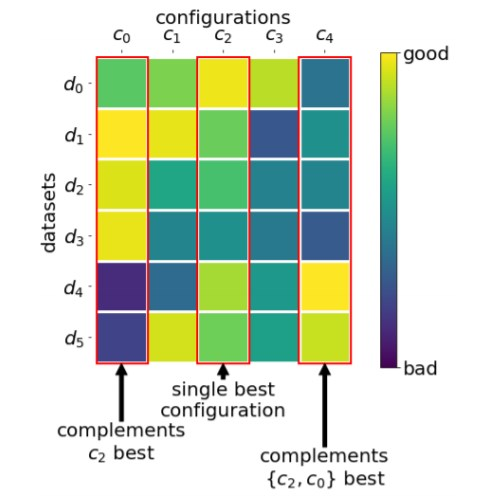
\includegraphics[width=.8\textwidth]{../w07_hpo_speedup/images/meta_learning/task_independent.jpg}}
%    \only<2->{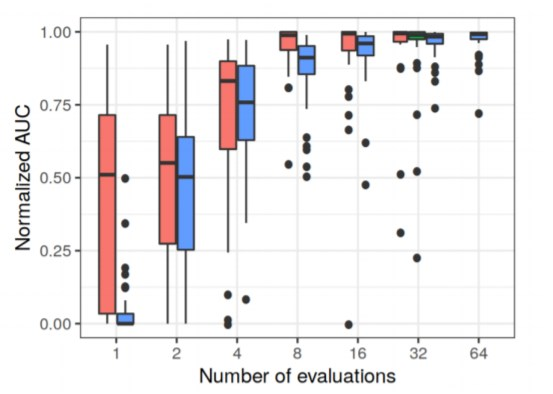
\includegraphics[width=.9\textwidth]{../w07_hpo_speedup/images/meta_learning/task_independent_results.jpg}}


\end{column}
\end{columns}  



\vspace{0.5cm}
\hspace{6cm}
\lit{\href{https://link.springer.com/article/10.1007/s10994-017-5684-y}{Wistuba et al. 2015a}}, \lit{\href{https://arxiv.org/pdf/1802.02219.pdf}{Feurer et al. 2018}},  \lit{\href{}{Pfisterer et al. 2018}}

}
%-----------------------------------------------------------------------
%-----------------------------------------------------------------------

%-----------------------------------------------------------------------
%-----------------------------------------------------------------------
\begin{frame}[c]{Meta-Learning for HPO Approach 4:\\ Joint model for Bayesian optimization}

\begin{columns}[T] % align columns
\begin{column}{.38\textwidth}

\begin{itemize}
    \item<1-> \alert{Jointly train} a ``deep'' neural network \alert{on all tasks} 
    \myit{
    	\item<2-> Have a separate output layer (head) for each task 
    	\item<2-> Each head is a Bayesian linear regression (recall DNGO)
    }
    \item<3-> This uses meta-learning for feature extraction on the hyperparameter configurations 
\end{itemize}
\end{column}%

\hfill%

\begin{column}{.58\textwidth}
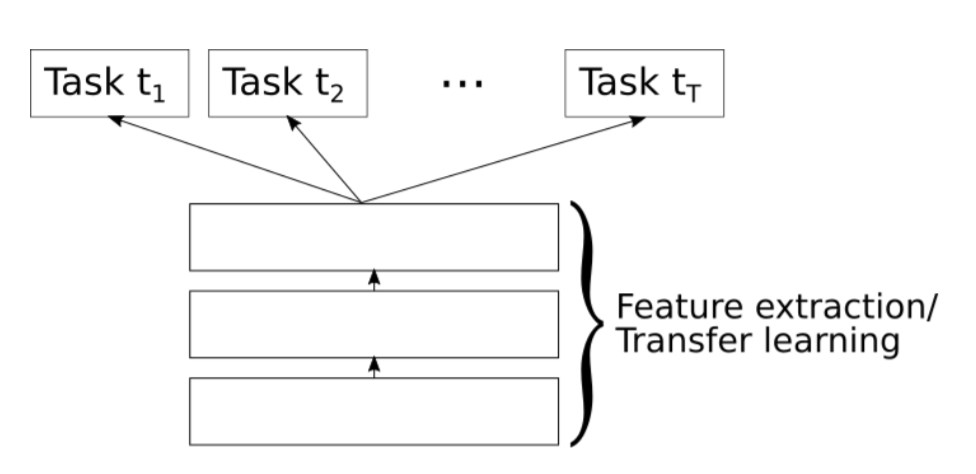
\includegraphics[width=0.9\textwidth]{../w07_hpo_speedup/images/meta_learning/perrone_int.jpg}
\end{column}%
\end{columns}

\hspace{12cm}\lit{\href{http://papers.nips.cc/paper/7917-scalable-hyperparameter-transfer-learning.pdf}{Perrone et al. 2018}}

\end{frame}
%-----------------------------------------------------------------------
%-----------------------------------------------------------------------
%\begin{frame}[c]{Joint model for Bayesian optimization}
%
%\centering
%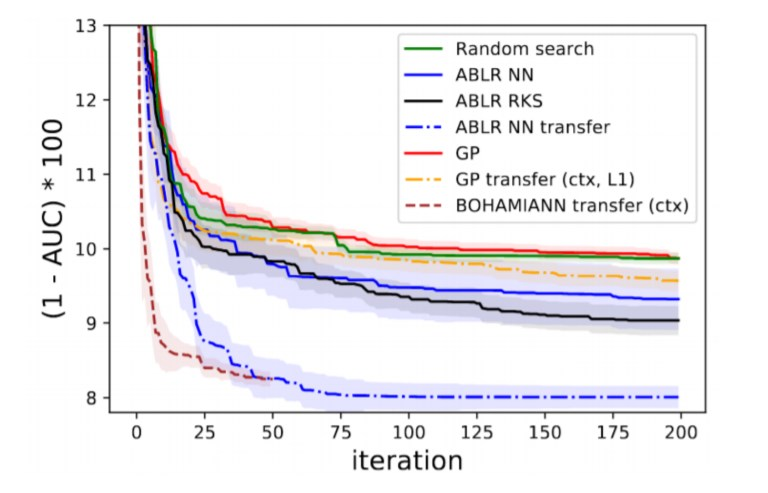
\includegraphics[width=0.7\textwidth]{../w07_hpo_speedup/images/meta_learning/perrone_res.jpg}
%
%\end{frame}
%-----------------------------------------------------------------------
%-----------------------------------------------------------------------

%----------------------------------------------------------------------
%----------------------------------------------------------------------
\begin{frame}[c]{Meta-Learning for HPO Approach 5:\\ Learning a Black-box Optimization Algorithm from Data}

\myit{

    \item \alert{Learning} a blackbox optimization algorithm
    \myit{
        \item Use $\dataset_{\text{meta}}$ to learn a mapping from $\dataset_{\text{new}}$ to the next configuration $\conf$ to evaluate
 %       \item This 
%        \item 
%        \cost_{i, \text{new}}$ on a new task $t_{\text{new}}$
 %       
 %       \iter[\bocount]{h}$ to next query $\iter[\bocount]{x}$
        \item This mapping can be a (recurrent) neural net $\text{NN}_{\phi}: \dataset_{\text{new}} \mapsto \conf$ parameterized by weights $\phi$   
\pause        
\smallskip
        \item \alert{This mapping $\text{NN}_{\phi}$ constitutes a blackbox optimization algorithm}
%        \myit{
%            \item Should be learned on a \alert{meta-train} set of blackbox functions \& generalize to new functions
%            \item Like a manually-designed algorithm ...
%        }

%\pause
%        \item Since $\iter[\bocount]{h}$ captures a \alert{sequence}, a recurrent NN $RNN_{\phi}:\iter[\bocount]{h} \mapsto \iter[\bocount]{x}$ makes sense

\pause
\bigskip
    
    }
    
    \item Existing approaches for learning a blackbox optimizer
    \myit{
        \item \alert{Gradient descent} on $\phi$  \lit{\href{http://proceedings.mlr.press/v70/chen17e.html}{Chen et al. 2017}}
        \myit{
            \item Simplest technique, but requires backpropagation through the optimization trace
            \item This also requires the blackbox functions $f$ used for training to be differentiable
       }
\pause
        \item \alert{Reinforcement learning} \lit{\href{https://arxiv.org/abs/1606.01885}{Li \& Malik, 2016}}
        \myit{
            \item Can be harder to get to work, but does not require differentiable $f$
        }
    
%        \item Gradient-free approaches should also work

    }
}

\end{frame}
%----------------------------------------------------------------------
%----------------------------------------------------------------------
%-----------------------------------------------------------------------
%-----------------------------------------------------------------------
\begin{frame}[c]{Meta-Learning for HPO Approach 6: Learning Algorithm Parts}

\begin{itemize}
	\item Learning a complete optimization algorithm  \alert{requires a lot of data}
	\item It would be more \alert{sample-efficient} to \alert{only replace hand-designed parts} of an algorithm

\bigskip
\pause
	\item In Bayesian optimization, a critical hand-designed heuristic is the acquisition function
	\begin{itemize}
		\item Trade-off between exploitation and exploration, e.g., via PI, EI, UCB, ES, KG, \dots 
		\item Depending on the problem at hand, you might need a different acquisition function
		%all of them are \alert{myopic} (no long-term look-ahead)
	\end{itemize}
\pause
\smallskip

    \item \alert{Idea:} Learn a \alert{neural acquisition function} from data, but still make use of the sample efficiency of Gaussian processes \lit{\href{https://openreview.net/forum?id=ryeYpJSKwr}{Volpp et al. 2020}}

\pause
\medskip
    \item Two options:
    \myit{
        \item Only depend on predicted mean and variance: $\acq_\phi(\conf) = \acq_\phi(\mu_t(\conf), \sigma_t(\conf))$ 
        \myit{
            \item This allows to learn a general acquisition function
        }
\pause
        \item Also depend on the $\conf$ value: $\acq_\phi(\conf) = \acq_\phi(\mu_t(\conf), \sigma_t(\conf), \alert{\conf})$  
        \myit{
            \item This allows to fine-tune to the characteristics of $\mathcal{D}_{\text{meta}}$ (e.g., avoid poor parts of the space) 
        }
    }

\end{itemize}


\end{frame}
%-----------------------------------------------------------------------

%-----------------------------------------------------------------------
\begin{frame}[c]{Questions to Answer for Yourself / Discuss with Friends}

\begin{itemize}
    \item \alert{Repetition.} What are the different kinds of meta-features which can be used to describe machine learning datasets?
    
    \medskip

    \item \alert{Repetition.} List all the different ways of using the meta data for HPO you recall
    \medskip

    \item \alert{Discussion.}
    \begin{itemize}
%        \item How would you pick meta-features to be used in meta-learning hyperparameter optimization?
        \item In the various meta-learning approaches, what will happen if all prior tasks are dissimilar to the target task?
    \end{itemize}


\end{itemize}

\end{frame}